
% \begin{figure}[ht]
%     \centering
%     \begin{subfigure}[t]{0.2\textwidth}
%         \centering
%         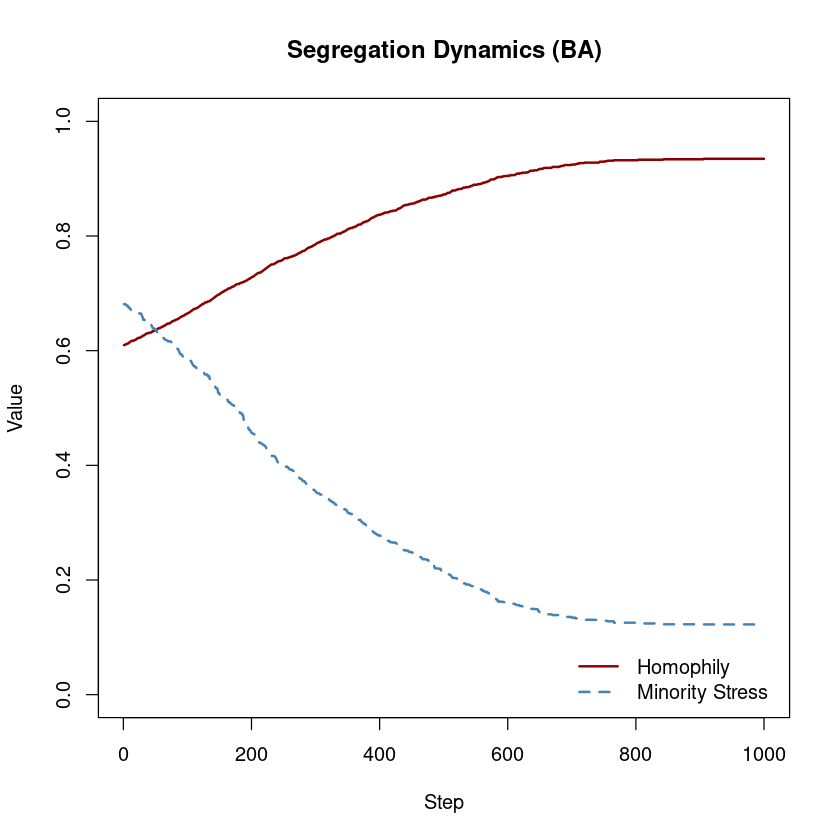
\includegraphics[width=\linewidth]{images/henryba.png}
%         \caption{Caption 1}
%     \end{subfigure}
%     \hfill
%     \begin{subfigure}[t]{0.2\textwidth}
%         \centering
%         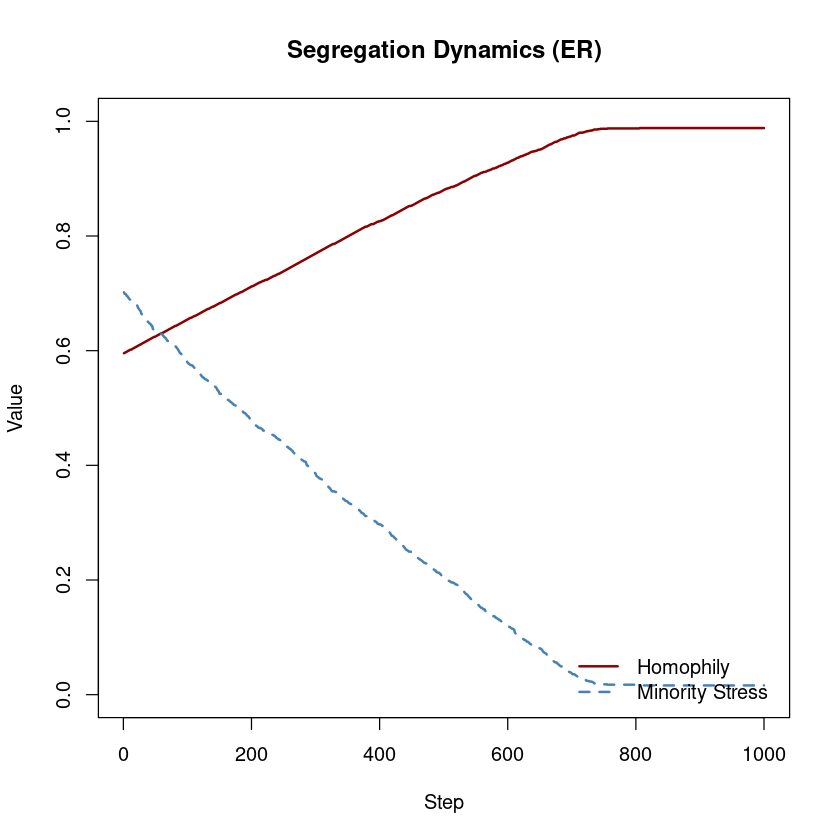
\includegraphics[width=\linewidth]{images/henryer.png}
%         \caption{Caption 2}
%     \end{subfigure}
%     \hfill
%     \begin{subfigure}[t]{0.2\textwidth}
%         \centering
%         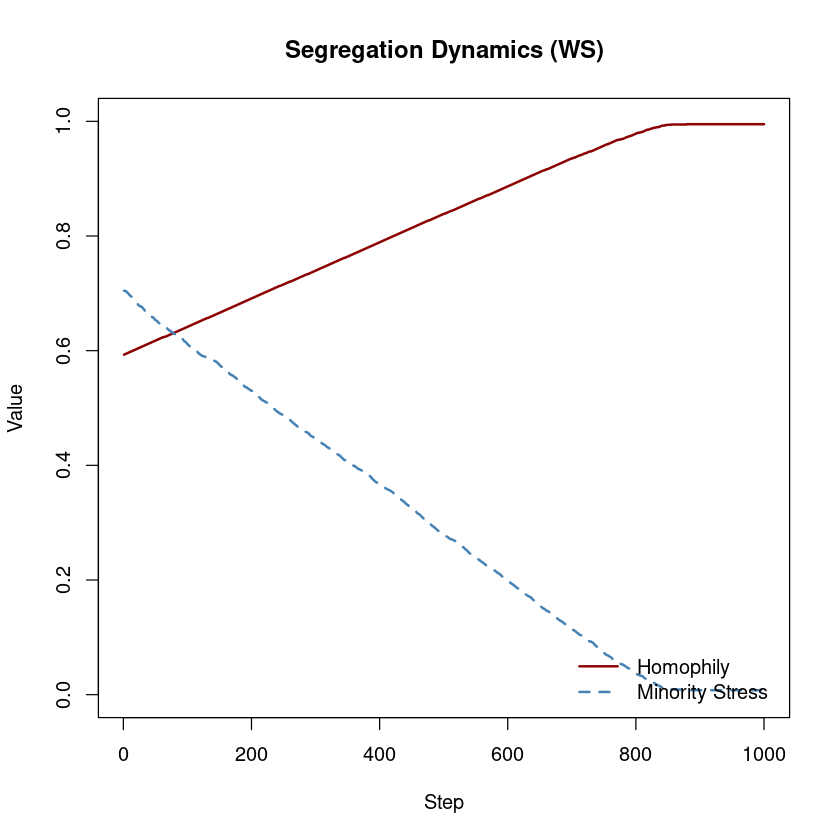
\includegraphics[width=\linewidth]{images/henryws.png}
%         \caption{Caption 3}
%     \end{subfigure}
%     \hfill
%     \begin{subfigure}[t]{0.2\textwidth}
%         \centering
%         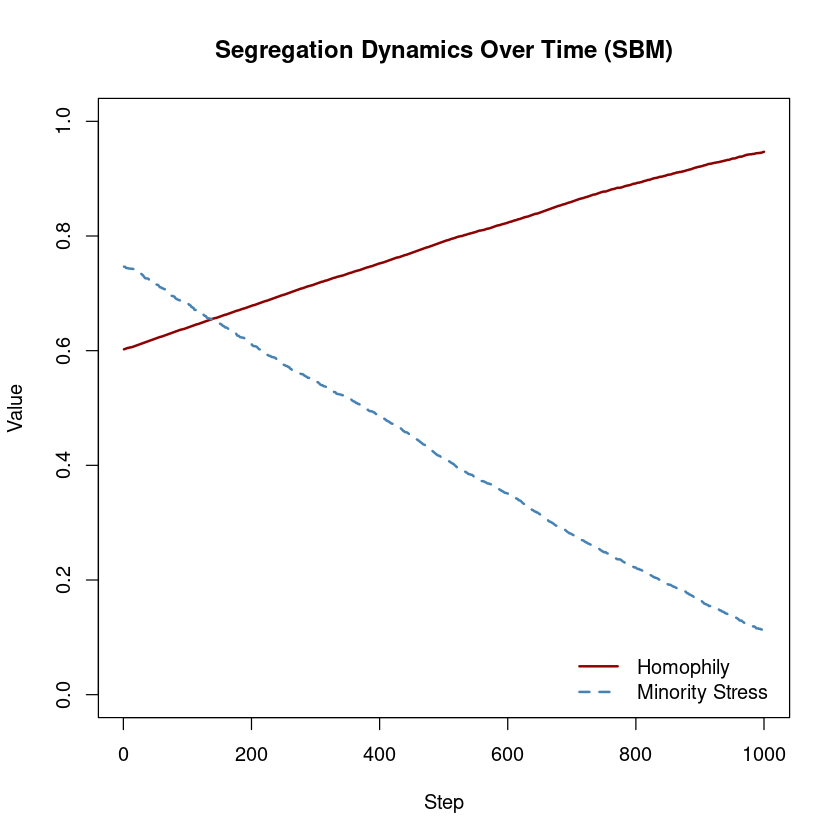
\includegraphics[width=\linewidth]{images/henrysbm.png}
%         \caption{Caption 4}
%     \end{subfigure}
%     \caption{Overall figure caption}
%     \label{fig:henry}
% \end{figure}




\begin{figure}[htbp]
    \centering
    \begin{minipage}[t]{0.24\linewidth}
        \centering
        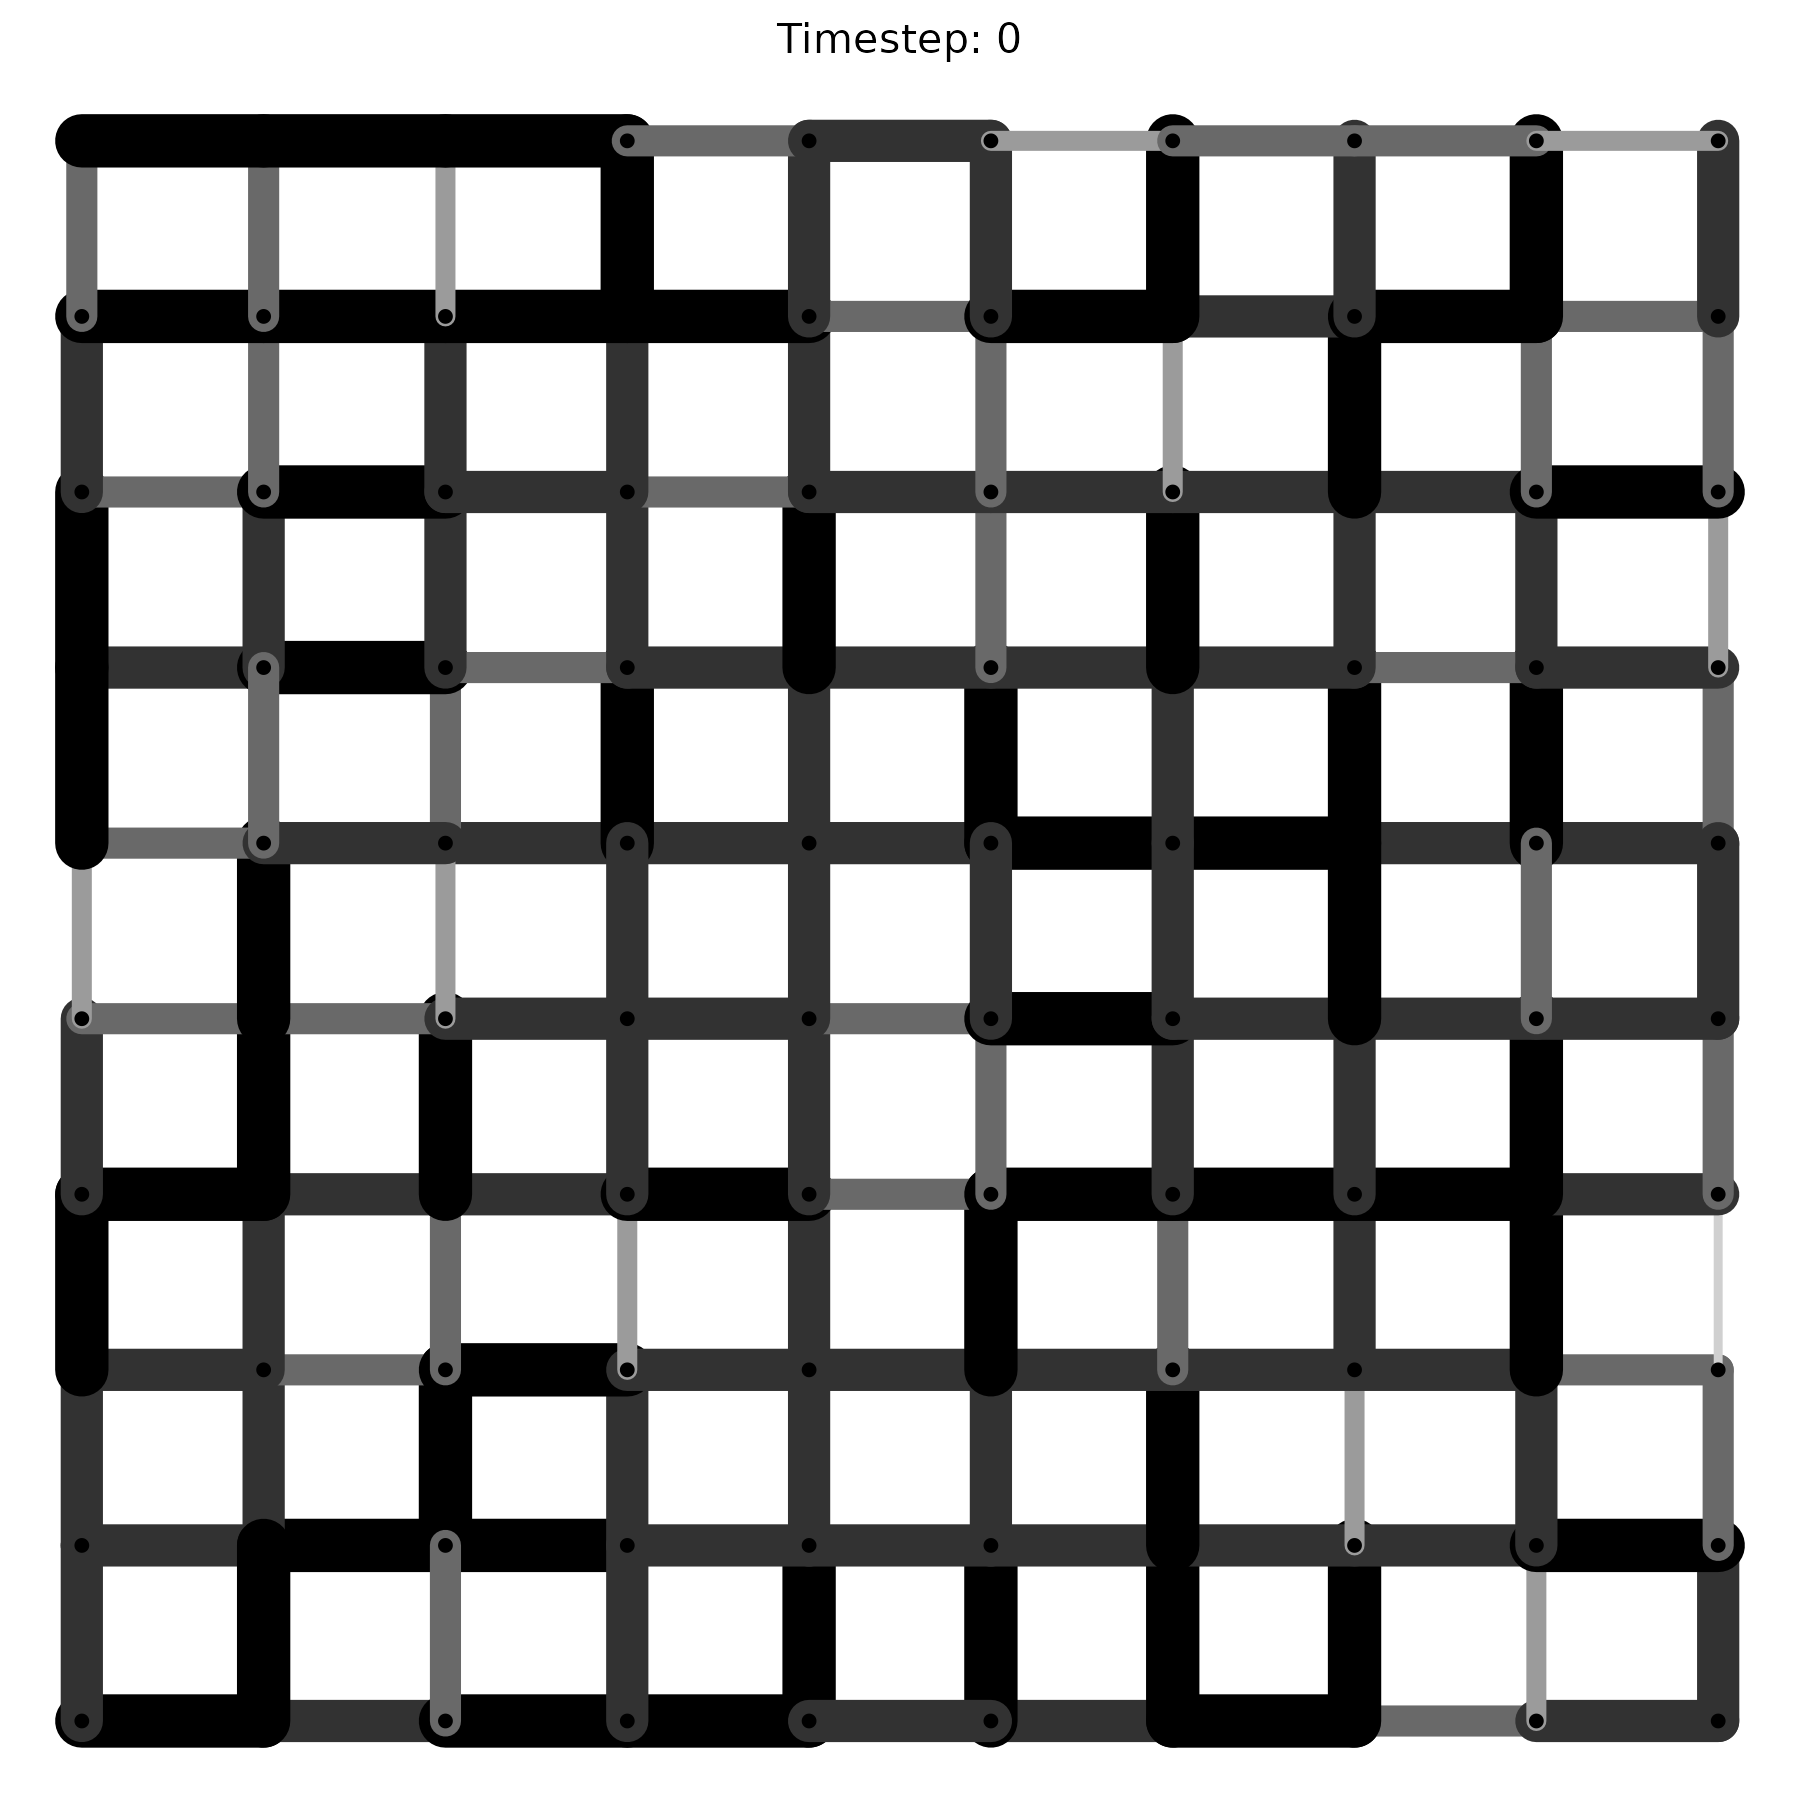
\includegraphics[width=\linewidth]{images/ax0.png}
        
    \end{minipage}
    \hfill
    \begin{minipage}[t]{0.24\linewidth}
        \centering
        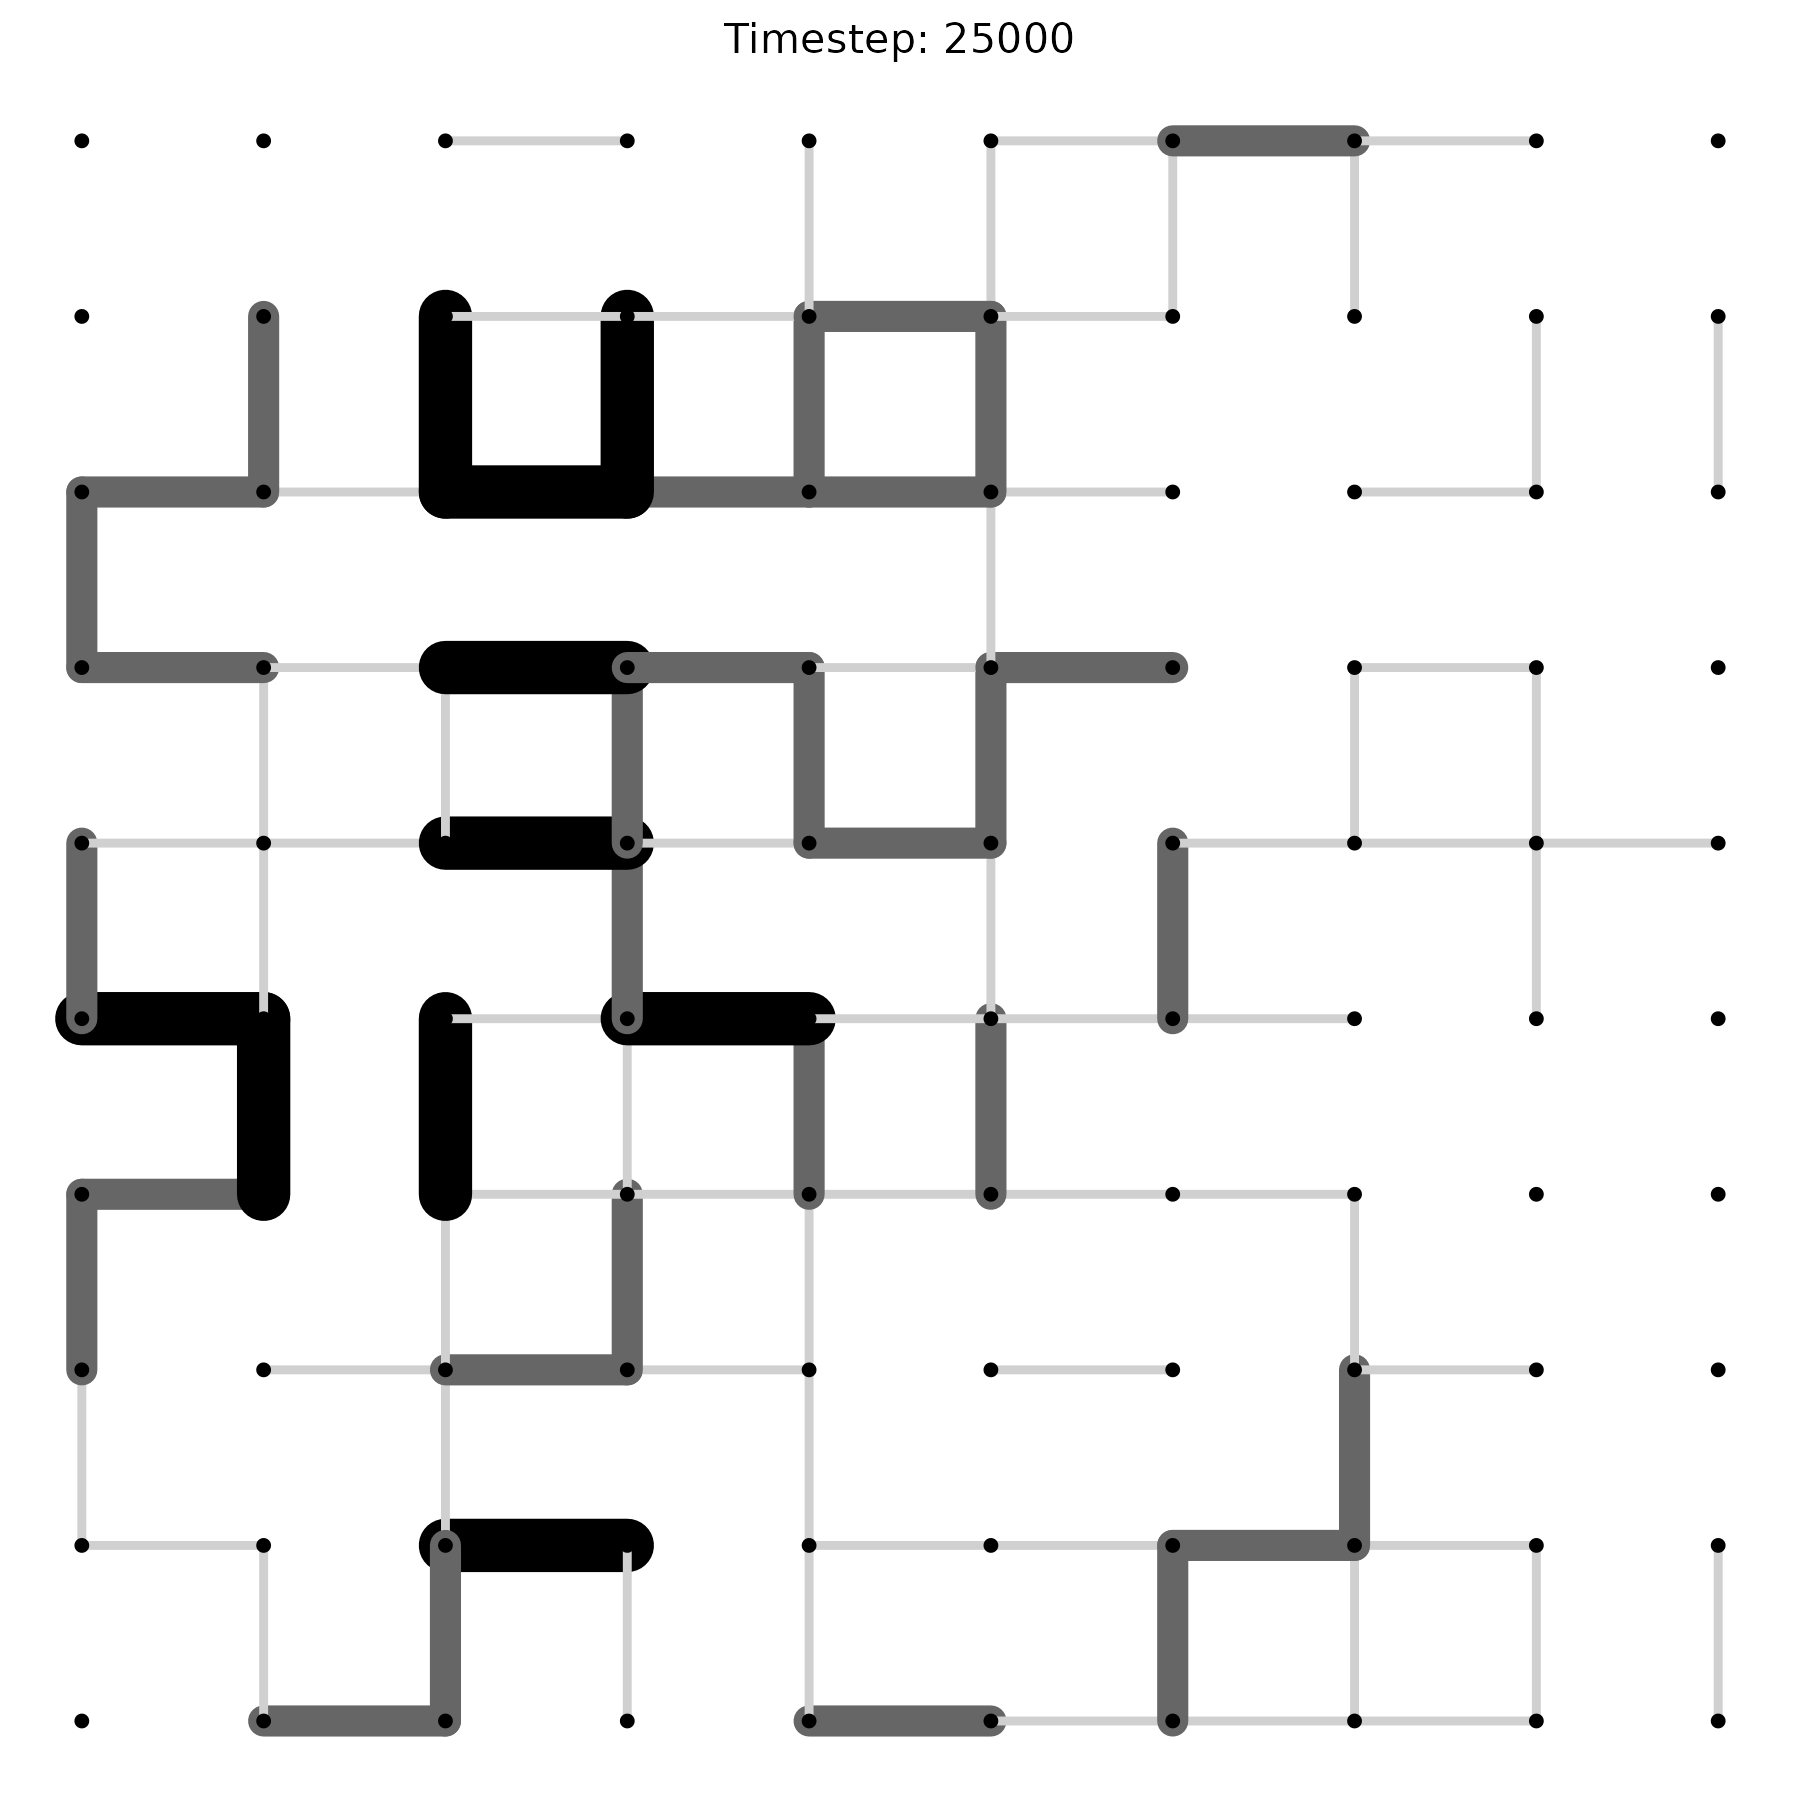
\includegraphics[width=\linewidth]{images/ax1.png}
        
    \end{minipage}
    \hfill
    \begin{minipage}[t]{0.24\linewidth}
        \centering
        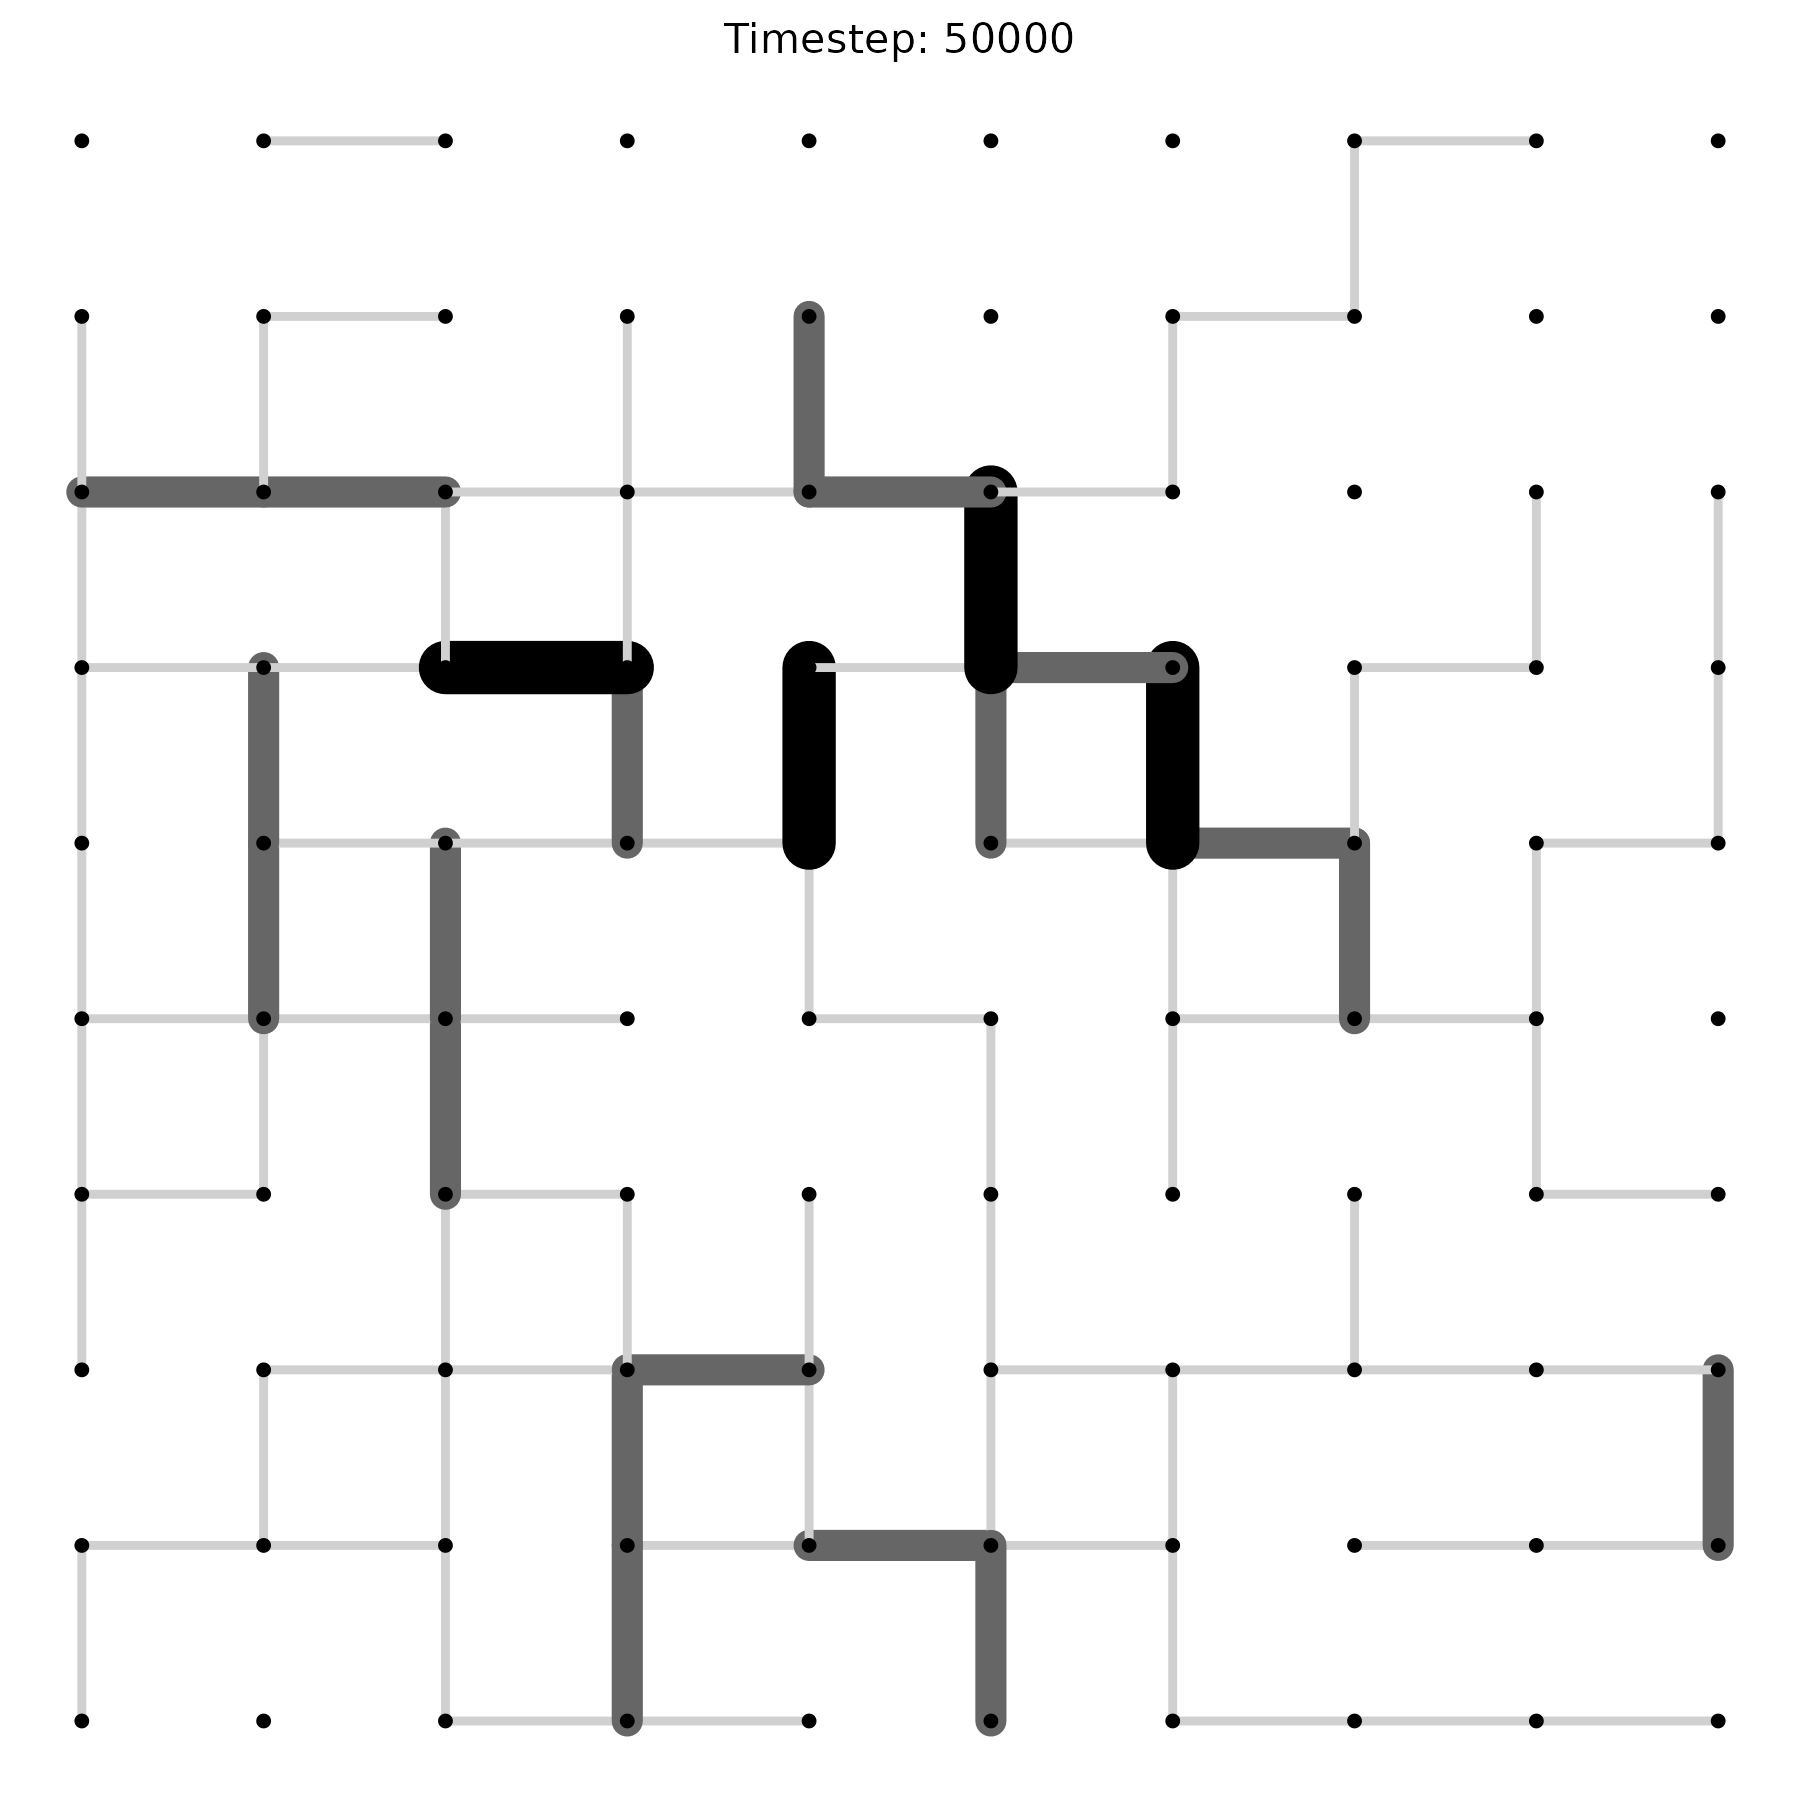
\includegraphics[width=\linewidth]{images/ax2.png}
        
    \end{minipage}
    \hfill
    \begin{minipage}[t]{0.24\linewidth}
        \centering
        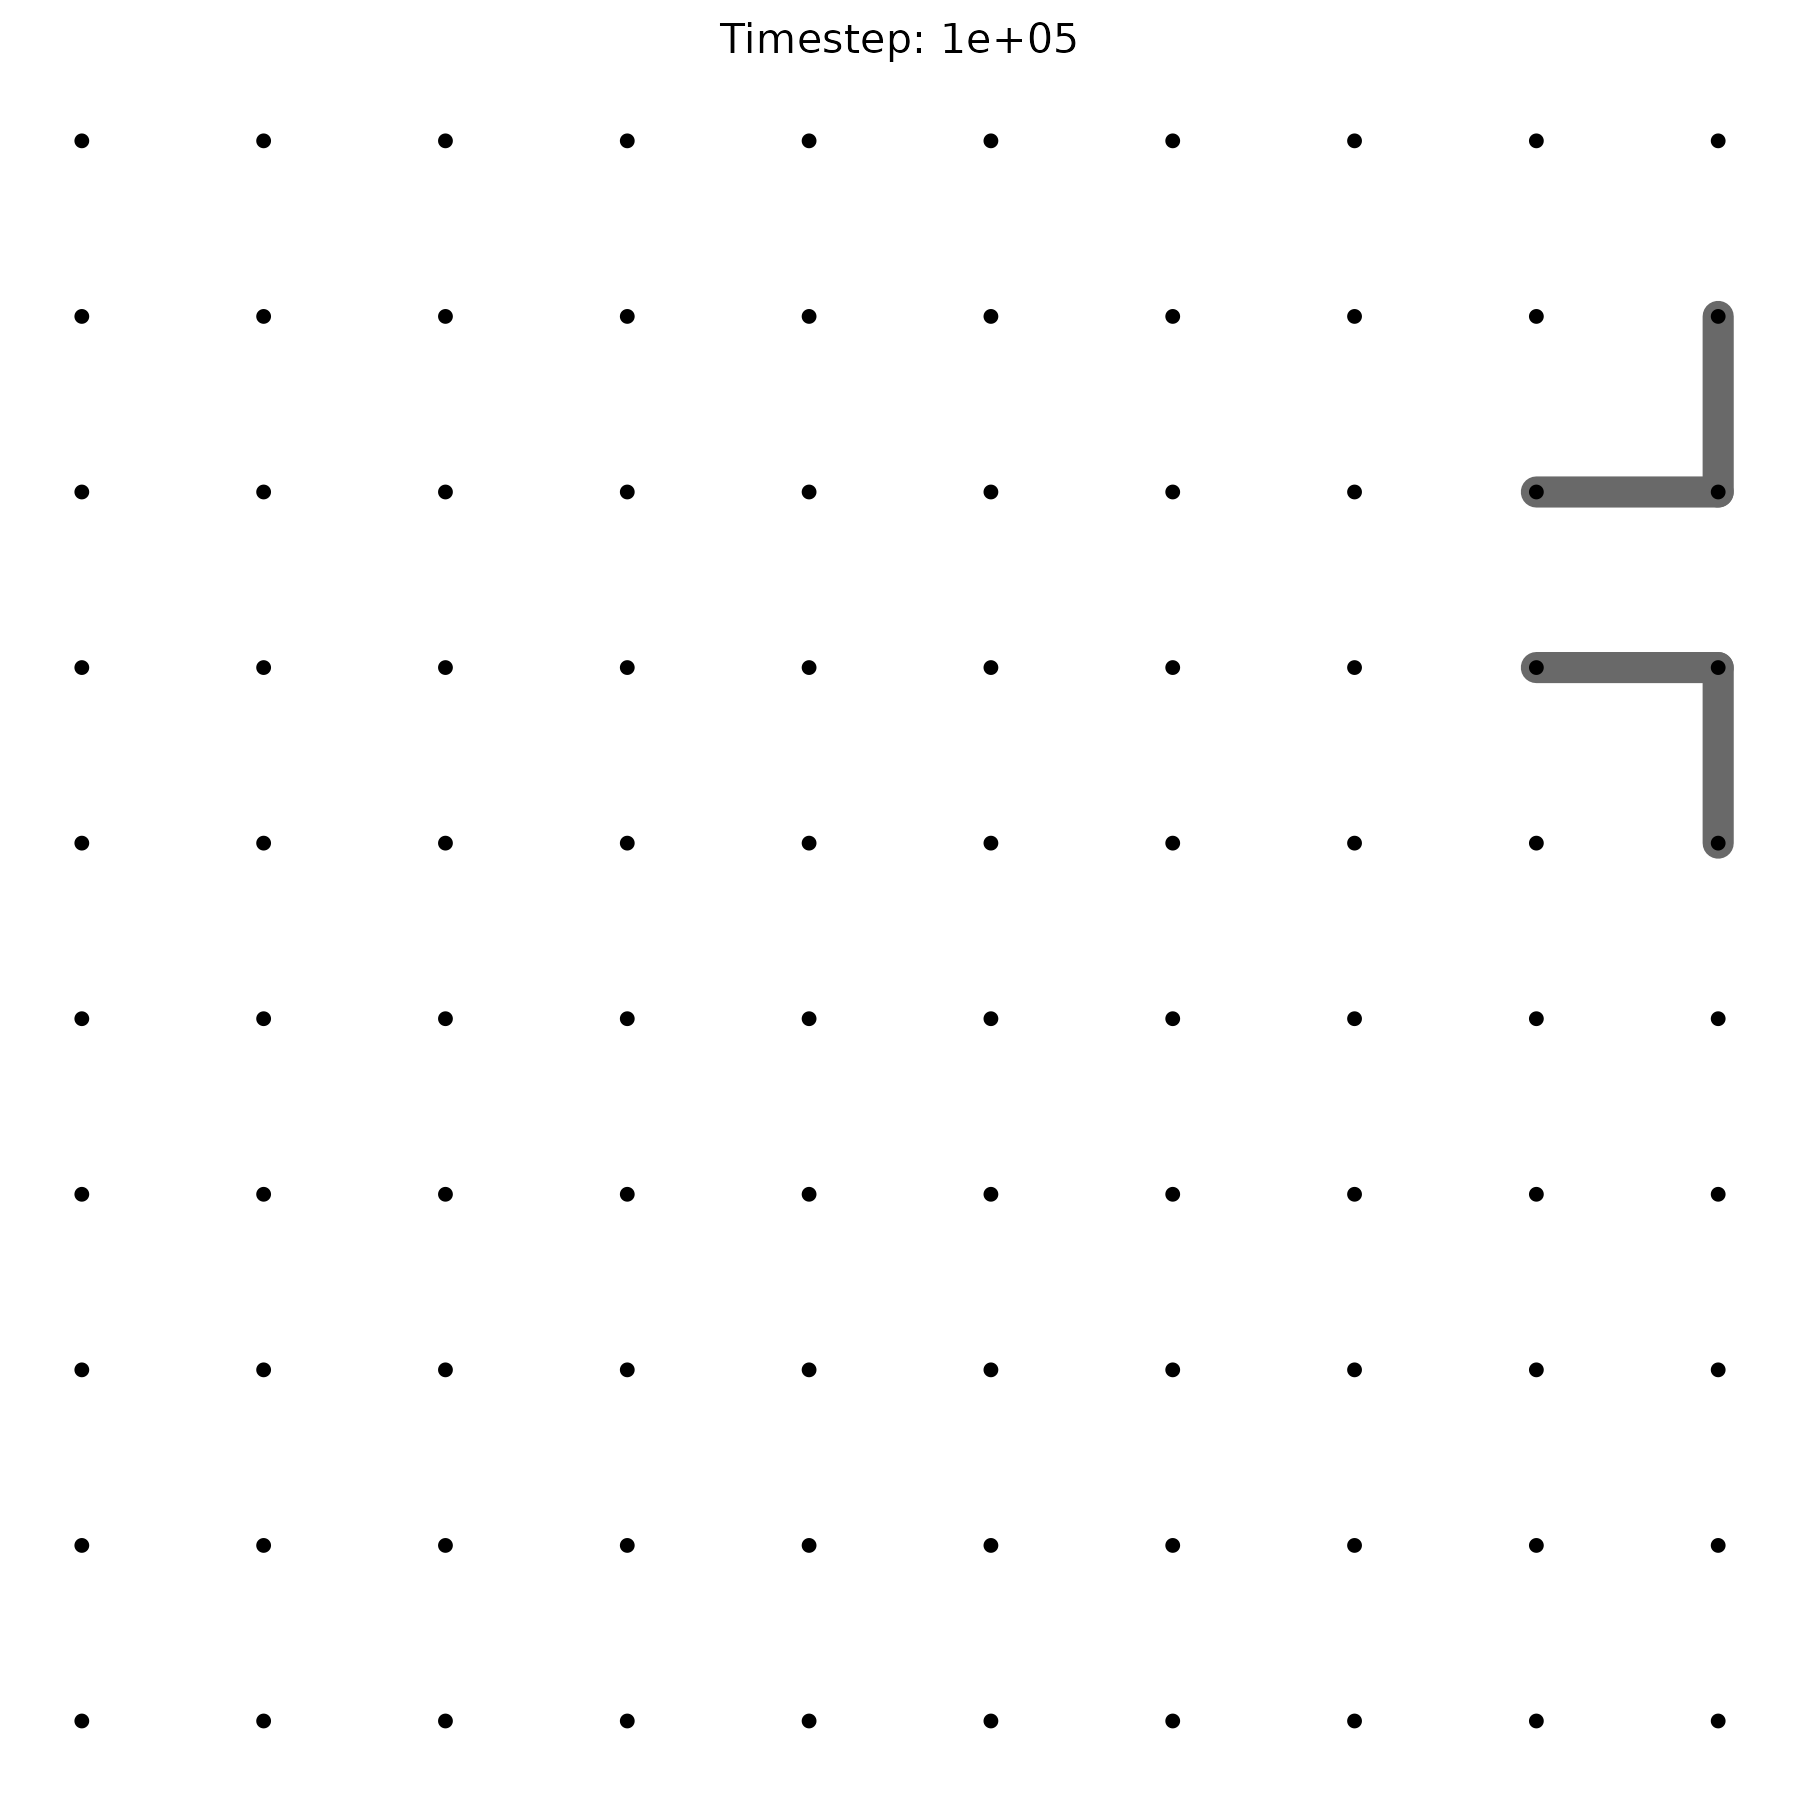
\includegraphics[width=\linewidth]{images/ax3.png}
        
    \end{minipage}
    \caption{Cultural diffusion at several iteration steps. Edges' thickness and darkness are proportional to the dissimilarity among the respective nodes. Timestep is specified on top of the respective figure.}
    \label{fig:ax}
\end{figure}
